\documentclass[11pt]{article}
\usepackage[margin=1in]{geometry}
\usepackage{amsmath, amssymb, amsthm}
\usepackage{graphicx}
\usepackage{xcolor}
\usepackage{hyperref}
\usepackage{algorithm}
\usepackage{algpseudocode}
\usepackage{setspace}
\usepackage{biblatex}
\usepackage{arydshln}
\usepackage{subcaption}
\setstretch{1.15}
\addbibresource{references.bib} %Import the bibliography file

\title{\textbf{paper yoyos quasi-static model}}
\author{Brandon Wong, Ben Foster}
\date{\today}

\begin{document}

\maketitle

\section{Simplified geometric model}\label{sec:setup}
\begin{figure}
    \centering
    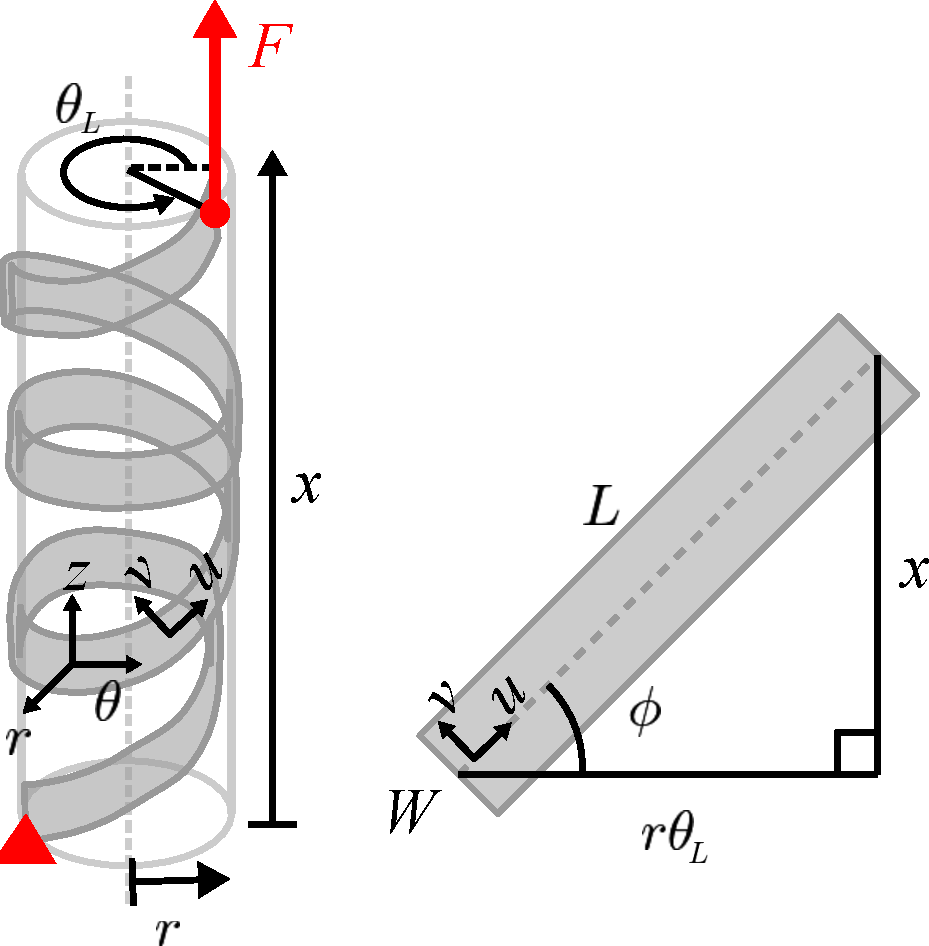
\includegraphics[width=0.5\textwidth]{figs/capstan_helix.pdf}
    \caption{in progress}\label{fig:setup}
\end{figure}

The system can be modelled as a constant-width rectangular ribbon of negligible thickness wrapped around a uniform-radius cylinder at a uniform pitch. One end of the ribbon is fixed in place (the ``base end'') to prevent rigid body motion, while the other (``active'' end) is displaced in the $z$ direction (the axis of the cylinder). Refer to Figure~\eqref{fig:setup} for a visual representation of the system. The system has the following geometric constants:
\begin{itemize}
    \item $L$: the length of the unrolled rectangle.
    \item $W$: the width of the unrolled rectangle. Assume $L \gg W$.
    \item $t$: the thickness of the material. Assume $L \gg W \gg t$.
    \item $\theta_L$: the total wind angle of the helix, which is fixed based on the boundary conditions (the two ends of the ribbon cannot rotate about the $z$-axis relative to one another, only translate along it, so the total number of turns is a fixed topological property of how the ribbon was wound and does not change as it is pulled). $\theta_L = 2\pi n$ where $n$ is the number of winds around the $z$ axis (not necessarily integer).
\end{itemize}

The state of the system is parametrized by the parameter $x$, which describes how far the active end has displaced in the $z$ direction relative to the base end.

Positions on the helix can be described with local surface $u,v$ coordinates, which describe the unrolled rectangle. The $u$ direction runs along the length of the unrolled rectangle, and the $v$ direction runs across its width. Alternatively, positions can be described in 3d space using cylindrical $r,\theta,z$ coordinates.

To simplify the geometry, we assume that the helix has a radius $r$ and a pitch angle $\phi$ (the angle the local $\hat{u}$ makes with the $r,\theta$ plane) relative to $u,v$ at any point in time. Equivalently, the local orthonormal frame $(\hat u,\hat v)$ tangent to the ribbon surface is related to the cylinder's own natural frame $(\hat\theta,\hat z)$ by a rotation through the angle $\phi$:
\begin{equation}\label{eq:frame_rotation}
    \hat u = \cos\phi\,\hat\theta + \sin\phi\,\hat z, \qquad
    \hat v = -\sin\phi\,\hat\theta + \cos\phi\,\hat z.
\end{equation}
($\hat v$ is obtained by rotating $\hat u$ a further $90^\circ$ around $\hat{r}$ in the same sense, so that $(\hat u,\hat v)$ remains a right-handed orthonormal frame like $(\hat\theta,\hat z)$.) Equation~\eqref{eq:frame_rotation} is the single geometric fact that determines everything else about the shape of the ribbon: because $\phi$ is just the angle between the ribbon's own axes and the cylinder's axes, every quantity that depends on this rotation will naturally involve $\cos\phi,\sin\phi$, and---once such quantities are combined pairwise, as stresses and curvatures are---their double-angle combinations $\cos^2\phi,\sin^2\phi, 2\sin\phi\cos\phi = \sin2\phi $. 

We now use Eq.~\eqref{eq:frame_rotation} to relate the geometric constants $L,\theta_L$ to the pitch angle $\phi$ and radius $r$ at a given extension $x$. From Eq.~\eqref{eq:frame_rotation}, $\hat u$ has $z$-component $\sin\phi$, so moving a distance $\mathrm du$ along the ribbon's own length produces an axial displacement $\mathrm dz=\sin\phi\,\mathrm du$. Since $\phi$ is constant along the whole ribbon at a given (frozen) extension $x$, integrating this from the base end ($u=0$) to the active end ($u=L$) gives a total axial displacement of $L\sin\phi$. By definition, this total axial displacement between the two ends of the ribbon is exactly $x$, so
\begin{equation}\label{eq:phi}
    x = L\sin\phi \qquad\Longrightarrow\qquad \phi = \sin^{-1}\left(\frac{x}{L}\right).
\end{equation}
Likewise, $\hat u$ has $\theta$-component $\cos\phi$, so moving a distance $\mathrm du$ along the ribbon produces a circumferential arc length $r\,\mathrm d\theta = \cos\phi\,\mathrm du$. Integrating over the whole ribbon length $L$, the ribbon sweeps out a total circumferential arc length $L\cos\phi$. This total arc length must also equal $r\theta_L$ (arc length equals radius times swept angle), since by construction the ribbon winds through the fixed total angle $\theta_L$ regardless of $x$. Equating the two expressions for this arc length and using $\cos\phi=\sqrt{1-\sin^2\phi}$ together with Eq.~\eqref{eq:phi} gives
\begin{equation}\label{eq:r}
    r\theta_L = L\cos\phi \qquad\Longrightarrow\qquad r = \frac{L}{\theta_L}\cos\phi = \frac{L}{\theta_L}\sqrt{1-\frac{x^2}{L^2}} = \frac{\sqrt{L^2 - x^2}}{\theta_L}.
\end{equation}
\section{Quasi-static Equilibrium}
We will model the paper yoyo as a 2d membrane. We will ignore stresses due to elastic deformation and will assume the kinematics are dominated by developable plastic bending deformation rather than in plane stretching.


\subsection{In-plane force balance}

An area element $du \times dv$ at point $(u,v)$ has a plane stress tensor:
\begin{equation}
    \sigma(u,v) = 
    \begin{bmatrix}
        \sigma_{uu} & \sigma_{uv}\\
        \sigma_{uv} & \sigma_{vv}
    \end{bmatrix}
\end{equation}

Now we perform a force balance on the area element in $u$ and $v$. We model the ribbon as a thin physical sheet of uniform thickness $t \ll W \ll L$. An area element of length $\mathrm{d}u$ and width $\mathrm{d}v$ has a volume $\mathrm{d}u \, \mathrm{d}v \, t$. Let $\boldsymbol{\sigma}(u,v)$ denote the 3D Cauchy plane-stress tensor acting within the membrane, with components $\sigma_{uu}$ and $\sigma_{uv}$ having dimensions of force per unit area ($\text{N/m}^2$). The in-plane membrane forces per unit length ($\text{N/m}$) transmitted across the faces of the differential element are therefore $\sigma_{uu}t$, $\sigma_{uv}t$, and $\sigma_{vv}t$.

The area element is not perfectly flat, but because $\cos\theta \approx 1$ for small angles, we can treat it as flat for the in-plane force balance. Let body forces due to friction $f_u,f_v$ denote the force components per unit volume in the $u$ and $v$ directions. The force balance in $u$ is:
\begin{align}
    \left[\sigma_{uv}(u,v+dv) - \sigma_{uv}(u,v)\right]t\,du + \left[\sigma_{uu}(u+du,v) - \sigma_{uu}(u,v)\right]t\,dv + f_u\, t\,du\, dv &= 0\\
    \frac{\sigma_{uv}(u,v+dv) - \sigma_{uv}(u,v)}{dv} + \frac{\sigma_{uu}(u+du,v) - \sigma_{uu}(u,v)}{du} + f_u &= 0
\end{align}
Dividing by $t$ and taking $du,dv\to0$ turns the difference quotients into partial derivatives:
\begin{equation}\label{eq:force_u}
    \boxed{\frac{\partial \sigma_{uv}}{\partial v} + \frac{\partial \sigma_{uu}}{\partial u} + f_u = 0}
\end{equation}
Repeating the identical bookkeeping for the force balance in the $v$ direction (now the two stress components entering are $\sigma_{uv}$, transmitted across the $u$-faces, and $\sigma_{vv}$, transmitted across the $v$-faces) gives, by the same steps,
\begin{equation}\label{eq:force_v}
    \boxed{\frac{\partial \sigma_{uv}}{\partial u} + \frac{\partial \sigma_{vv}}{\partial v} + f_v = 0}
\end{equation}

\subsection{Out-of-plane force balance}\label{sec:outofplane}
The in-plane force balance above treats the area element as flat, but the element is actually curved: it is wrapped around a cylinder of radius $r$, so the local frame $(\hat u,\hat v)$ tilts slightly as one moves from one face of the element to the opposite face. This tilt means that even a spatially uniform in-plane stress produces a net force component in the radial direction $\hat r$---exactly as, for instance, uniform tension in a curved rope produces a net inward force. We now compute this radial force and balance it against the contact pressure between adjacent, overlapping wound layers of the ribbon.

\subsubsection{Local frame rotation rates} 
A cylinder of radius $r$ has two principal curvatures: $\kappa_\theta = 1/r$ in the circumferential ($\hat\theta$) direction, and $\kappa_z = 0$ in the axial ($\hat z$) direction. For a tangent direction that makes angle $\alpha$ with the $\hat\theta$-direction, Euler's theorem for the normal curvature of a surface states that the rate at which a unit tangent vector pointing in that direction tilts toward the surface normal $\hat r$, per unit distance traveled in that direction, is
\begin{equation}\label{eq:euler}
    \kappa(\alpha) = \kappa_\theta\cos^2\alpha + \kappa_z\sin^2\alpha = \frac{\cos^2\alpha}{r}.
\end{equation}
% (This is the same fact, applied to curvature instead of stress, that underlies Mohr's circle: a symmetric rank-two tensor---here the shape operator, with eigenvalues $\kappa_\theta,\kappa_z$ along the orthogonal directions $\hat\theta,\hat z$---evaluated in a direction rotated by angle $\alpha$ from a principal axis always produces this $\cos^2\alpha,\sin^2\alpha$ combination; the associated off-diagonal, ``twisting'' rate between two directions at $90^\circ$ to each other is $(\kappa_\theta-\kappa_z)\sin\alpha\cos\alpha$.)

From Eq.~\eqref{eq:frame_rotation}, $\hat u$ is at angle $\phi$ from $\hat\theta$, and $\hat v$ is at angle $\phi+90^\circ$ from $\hat\theta$. Substituting $\alpha=\phi$ and $\alpha=\phi+90^\circ$ into Eq.~\eqref{eq:euler} (and using $\cos(\phi+90^\circ)=-\sin\phi$) gives the two diagonal rotation rates, and the off-diagonal formula gives the twisting rate between $\hat u$ and $\hat v$:
\begin{equation}\label{eq:curvatures}
    \kappa_{uu} = \frac{\cos^2\phi}{r}, \qquad
    \kappa_{vv} = \frac{\sin^2\phi}{r}, \qquad
    \kappa_{uv} = \frac{\sin\phi\cos\phi}{r}.
\end{equation}
Concretely, this means that, evaluating the differential rotation of the Darboux frame over the steps $\mathrm du$ and $\mathrm dv$:
\begin{itemize}
    \item On the $u+\mathrm{d}u$ face, $\hat{u}$ rotates inward (toward $\hat r$) by an angle $\kappa_{uu}\,\mathrm{d}u = \frac{\cos^2\phi}{r} \mathrm{d}u$, contributing a radial force of $-\left(\sigma_{uu} t \, \mathrm{d}v\right) \frac{\cos^2\phi}{r} \mathrm{d}u$.
    \item On the $u+\mathrm{d}u$ face, $\hat{v}$ rotates outward by $-\kappa_{uv}\,\mathrm du = -\frac{\sin\phi\cos\phi}{r} \mathrm{d}u$, contributing $\left(\sigma_{uv} t \, \mathrm{d}v\right) \frac{\sin\phi\cos\phi}{r} \mathrm{d}u$.
    \item On the $v+\mathrm{d}v$ face, $\hat{v}$ rotates inward by an angle $\kappa_{vv}\,\mathrm dv = \frac{\sin^2\phi}{r} \mathrm{d}v$, contributing a radial force of $-\left(\sigma_{vv} t \, \mathrm{d}u\right) \frac{\sin^2\phi}{r} \mathrm{d}v$.
    \item On the $v+\mathrm{d}v$ face, $\hat{u}$ rotates outward by $-\kappa_{uv}\,\mathrm dv = -\frac{\sin\phi\cos\phi}{r} \mathrm{d}v$, contributing $\left(\sigma_{uv} t \, \mathrm{d}u\right) \frac{\sin\phi\cos\phi}{r} \mathrm{d}v$.
\end{itemize}

\subsubsection{Contact pressure balance} 
We balance the net radial projection of these internal membrane forces against the inward clamping force exerted by overlapping adjacent layers. To express this balance directly in terms of quantities with Cauchy stress dimensions ($\text{N/m}^2$) and eliminate explicit dependence on membrane thickness $t$, we define the effective normal clamping pressure $P$. Balancing the forces across the volume element (summing the four contributions above together with the clamping pressure's own contribution, $\frac{Pt\mathrm du\,\mathrm dv}{r}$, which is the force per unit area $P$ exerted over the element's own footprint $t\,\mathrm du\,\mathrm dv$ divided by the same radius factor) yields:
\begin{equation}
    \frac{Pt\mathrm du\,\mathrm dv}{r} - \sigma_{uu} t \left(\frac{\cos^2\phi}{r}\right) \mathrm{d}u \, \mathrm{d}v - \sigma_{vv} t \left(\frac{\sin^2\phi}{r}\right) \mathrm{d}u \, \mathrm{d}v + 2 \sigma_{uv} t \left(\frac{\sin\phi\cos\phi}{r}\right) \mathrm{d}u \, \mathrm{d}v = 0
\end{equation}
Dividing through by the common geometric volume factor $\frac{t\mathrm du\,\mathrm dv}{r}$ directly isolates the effective clamping pressure $P$ (and, using $2\sin\phi\cos\phi=\sin2\phi$, writes the cross term compactly):
\begin{equation}\label{eq:p}
    \boxed{P = \sigma_{uu} \cos^2\phi + \sigma_{vv} \sin^2\phi - \sigma_{uv} \sin(2\phi)}
\end{equation}
% Substituting the global kinematic relations $\cos^2\phi = 1 - (x/L)^2$, $\sin^2\phi = (x/L)^2$, and $2\cos\phi\sin\phi = 2(x/L)\sqrt{1 - (x/L)^2}$ from Equations~(\eqref{eq:phi}) and (\eqref{eq:r}), we obtain:
% \begin{equation}
%     \boxed{P = \left(1 - \frac{x^2}{L^2}\right)\sigma_{uu} + \left(\frac{x^2}{L^2}\right)\sigma_{vv} - \left(\frac{2x}{L^2}\sqrt{L^2-x^2}\right)\sigma_{uv}}
% \end{equation}

\begin{figure}
\centering
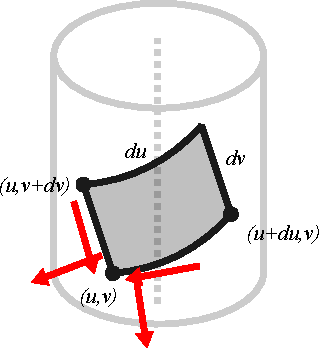
\includegraphics[width=0.5\textwidth]{figs/curved_element.pdf}
\caption{in progress}\label{fig:curved_element}
\end{figure}

\section{Friction}\label{sec:friction}

\subsection{Position and velocity of a ribbon element}
An area element $du \times dv$ at point $(u,v)$ has a position vector given in cylindrical coordinates. We build this up from Eq.~\eqref{eq:frame_rotation}: since $\hat u = \cos\phi\,\hat\theta+\sin\phi\,\hat z$, moving along the ribbon by $\mathrm du$ produces $r\,\mathrm d\theta = \cos\phi\,\mathrm du$ and $\mathrm dz = \sin\phi\,\mathrm du$; since $\hat v = -\sin\phi\,\hat\theta + \cos\phi\,\hat z$, moving across the width by $\mathrm dv$ produces $r\,\mathrm d\theta = -\sin\phi\,\mathrm dv$ and $\mathrm dz=\cos\phi\,\mathrm dv$. Integrating these (at a fixed $x$, so $r$ and $\phi$ are constants with respect to $u,v$) from the reference point $(u,v)=(0,0)$ gives
\begin{equation}
    \vec{p}(u,v,x) =
    \begin{bmatrix}
        r\\
        \theta\\
        z
    \end{bmatrix} =
    \begin{bmatrix}
        \frac{\sqrt{L^2-x^2}}{\theta_L}\\
        \frac{u \cos\phi - v \sin\phi}{r}\\
        u \sin\phi + v \cos\phi
    \end{bmatrix},
\end{equation}
% which, substituting $\sin\phi=x/L$, $\cos\phi=\sqrt{L^2-x^2}/L$ (Eq.~\eqref{eq:phi}) and $r=\sqrt{L^2-x^2}/\theta_L$ (Eq.~\eqref{eq:r}), is equivalently
which, substituting Eq.~\eqref{eq:phi} and Eq.~\eqref{eq:r} to expose the dependencies on $x$, is equivalently
\begin{equation}\label{eq:position}
    \vec{p}(u,v,x) =
    \begin{bmatrix}
        \frac{\sqrt{L^2 -x^2 }}{\theta_L }\\
        \frac{u\theta_L}{L}-\frac{v\,x\,\theta_L}{L\sqrt{L^2 -x^2 }}\\
        \frac{ux}{L}+\frac{v\sqrt{L^2 -x^2 }}{L}
    \end{bmatrix}.
\end{equation}
The velocity of a given material point $(u,v)$ as the active end of the ribbon is displaced (i.e., as $x$ changes) is then obtained by taking the partial derivative of each component of Eq.~\eqref{eq:position} with respect to $x$:

\begin{equation}\label{eq:velocity}
    \frac{\partial}{\partial x} \vec{p}(u,v,x) =
    \begin{bmatrix}
        \frac{\partial r}{\partial x}\\
        \frac{\partial \theta}{\partial x}\\
        \frac{\partial z}{\partial x}
    \end{bmatrix}=
    \begin{bmatrix}
        -\frac{x}{\theta_L \,\sqrt{L^2 -x^2 }}\\
        -\frac{L\,\theta_L\,v}{{\left(L^2-x^2\right)}^{3/2}}\\
        \frac{u}{L}-\frac{vx}{L\sqrt{L^2 -x^2 }}\\
    \end{bmatrix}.
\end{equation}

\subsection{Overlapping neighbors and the relative slip direction}
Because the ribbon is wound in a helix, a given area element at $(u,v)$ may physically overlap with other area elements one full turn away along the ribbon. Specifically, an area element at point $(u,v)$ overlaps with the neighboring interior layer at point $(u^-,v^-)$ if their cylindrical coordinates have equal $r$ and $z$, but differ by one full turn in $\theta$, i.e., $\theta(u^-,v^-) = \theta(u,v) - 2\pi$. Writing $\Delta u := u^- - u$ and $\Delta v:=v^--v$, and using $\vec{p}(u,v)$ from Eq.~\eqref{eq:position}, the two conditions $\theta(u^-,v^-)=\theta(u,v)-2\pi$ and $z(u^-,v^-)=z(u,v)$ become the linear system
\begin{align}
    \Delta u\cos\phi - \Delta v\sin\phi &= -2\pi r\\
    \Delta u\sin\phi + \Delta v\cos\phi &= 0
\end{align}
The second equation gives $\Delta u = -\Delta v\cos\phi/\sin\phi$; substituting into the first gives $-\Delta v(\cos^2\phi/\sin\phi) - \Delta v\sin\phi = -2\pi r$, i.e., $-\Delta v(\cos^2\phi+\sin^2\phi)/\sin\phi = -2\pi r$, i.e., $\Delta v = 2\pi r\sin\phi$, and then $\Delta u = -2\pi r\cos\phi$. Therefore,
\begin{align}
    u^- &= u - 2\pi r \cos \phi\\
    v^- &= v + 2\pi r \sin \phi \label{eq:vminus}
\end{align}
By the identical argument with $\theta(u^+,v^+)=\theta(u,v)+2\pi$ (i.e., the neighboring \emph{outer} layer, one full turn further out), the element has an outer overlapping neighbor at
\begin{align}
    u^+ &= u + 2\pi r \cos \phi\\
    v^+ &= v - 2\pi r \sin \phi
\end{align}

We can then plug $u^-,v^-$ into Eq.~\eqref{eq:velocity} to compute the velocity of the element relative to its inner overlapping neighbor, which gives the relative slip direction in the $r,\theta,z$ frame. Because $r$ and $z$ (by construction) agree for the two overlapping points, only the $\theta$-component of Eq.~\eqref{eq:velocity} actually differs between them; substituting $(u^-,v^-)$ into Eq.~\eqref{eq:velocity} and subtracting gives
\begin{equation}
    \frac{\partial \vec{p}(u,v,x)}{\partial x} - \frac{\partial \vec{p}(u^-,v^-,x)}{\partial x} =
    \begin{bmatrix}
        0\\
        \frac{2\pi\,x}{L^2-x^2}\\
        \frac{2\pi}{\theta_L}
    \end{bmatrix}.
\end{equation}
As expected, there is no relative velocity in the radial direction (i.e., the layers are not lifting away from each other). We can now compute the relative slip direction in the local $u,v$ frame by projecting this slip velocity onto the local basis vectors defined in Eq.~\eqref{eq:frame_rotation}. Since the $\frac{\partial \theta}{\partial x}$ component of $\frac{\partial \vec{p}}{\partial x}$ above is an \emph{angular} rate, we first convert it to a linear (arc-length) rate by multiplying by $r$, then projecting as just described:
\begin{equation}\label{eq:vslip_raw}
    \vec{v}_{slip}(u,v,x) = \begin{bmatrix}
        \cos\phi & \sin\phi \\
        -\sin\phi & \cos\phi
    \end{bmatrix}
    \begin{bmatrix}
        r\cdot\frac{2\pi\,x}{L^2-x^2}\\
        \frac{2\pi}{\theta_L}
    \end{bmatrix} 
\end{equation}
We simplify this expression by substituting subsituting $x$ and $r$ in terms of $\phi$ (Eq.~\eqref{eq:phi},~\eqref{eq:r}) to expose the double-angle combination, then applying double angle trig identities to factor out common terms. The result is a scaled unit vector:
\begin{equation}
    \vec{v}_{slip}(u,v,x) = \frac{2\pi}{\theta_L\cos\phi} \begin{bmatrix} \sin(2\phi) \\ \cos(2\phi) \end{bmatrix}
\end{equation}
The prefactor is strictly positive for all $x \in (0,L)$. Therefore, the relative slip velocity points in the direction of the unit vector $-(\sin2\phi,\cos2\phi)$ in the local $u,v$ frame, so the Coulomb friction force opposing this motion must point in the opposite direction:
\begin{equation}\label{eq:friction_direction}
    \hat{f} = -\begin{bmatrix} \sin(2\phi) \\ \cos(2\phi) \end{bmatrix}
\end{equation}

\subsection{Net frictional body force}
To compute the magnitude of the net frictional body force on the area element, we must evaluate the surface normal forces applied from both the top and bottom faces. Let $P_{out}(u,v)$ be the radial clamping pressure exerted inwards by the outer neighbor, and $P_{in}(u,v)$ be the reaction pressure exerted outwards by the inner neighbor. For the membrane element to maintain radial equilibrium, the inner layer must support both the outer clamping pressure and the element's own curvature-induced pressure $P$ (defined in Equation~\eqref{eq:p}), which is essentially the $\hat{r}$ components of the total stress tensor. Thus, the radial balance is:
\begin{equation}
    P_{in} = P_{out} + P
\end{equation}

The external pressures are non-negative in their defined directions, because a surface can only push, not pull, on its neighboring surfaces. The curvature-induced pressure $P$ is also assumed to be non-negative because the system as a whole is under tension. Therefore, if an element has no inner neighbor, then 
\begin{equation}
    P_{in} = 0 \quad\Longrightarrow\quad P_{out} + P = 0 \quad\Longrightarrow\quad P_{out} = 0
\end{equation}
and there is no friction force acting on the element. This is the ``overhang'' case, where the element is unsupported from the inside and cannot sustain any contact pressure at all, regardless of outer layer contact.

Alternatively, if an element does have an inner neighbor, then the area element slips forward relative to its inner neighbor along the slip direction $\vec{v}_{slip}$. Consequently, the inner neighbor exerts a frictional drag force that opposes this motion, with a magnitude proportional to $P_{in}$. Simultaneously, the outer neighbor is also slipping forward relative to the current element. By Newton's Third Law, the outer layer drags the current area element forward, with a magnitude proportional to $P_{out}$. It may be the case that $P_{out} = 0$ if there is no outer neighbor. Then, the net frictional resistance per unit volume opposing the element's motion is the difference between the backward drag of the inner layer and the forward drag of the outer layer:
\begin{equation}\label{eq:f_magnitude}
    f_{net} = \frac{\mu}{r} \left( P_{in} - P_{out} \right) = \frac{\mu}{r} \left( P_{out} + P - P_{out} \right) = \frac{\mu P}{r}
\end{equation}
In this case, the external pressures cancel, so the net friction driving the tension gradient in any supported element depends only on its own geometric pressure contribution $P$.


% \subsubsection{Net frictional body force}
% To compute the magnitude of the net frictional body force on the area element, we must evaluate the surface normal forces applied from both the inner and outer faces. Let $P_{out}(u,v)$ be the radial clamping pressure exerted inwards by the outer neighbor, and $P_{in}(u,v)$ be the reaction pressure exerted outwards by the inner neighbor, at a location where such a neighbor is present. For an element resting against an inner neighbor, radial equilibrium requires that neighbor to support both the outer clamping pressure and the element's own curvature-induced pressure $P$ (defined in Eq.~\eqref{eq:p}), which is essentially the $\hat r$-component of the total stress tensor:
% \begin{equation}\label{eq:Pin_eq}
%     P_{in} = P_{out} + P, \qquad\text{wherever an inner neighbor is present.}
% \end{equation}
% The external pressures $P_{in},P_{out}$ are non-negative in their defined directions, because a surface can only push, not pull, on its neighboring surfaces; we likewise take $P\ge0$, a claim we defer to Section~\ref{sec:closed_form} (Eq.~\ref{eq:P_nonneg_proof}) to justify rigorously.
 
% If an element does have an inner neighbor, it slips forward relative to it along the slip direction $\vec v_{slip}$, so the inner neighbor exerts a frictional drag force opposing this motion, with magnitude proportional to $P_{in}$; simultaneously, if an outer neighbor is present, it is itself slipping forward relative to the current element, so by Newton's Third Law it drags the current element forward, with magnitude proportional to $P_{out}$ (which is simply zero if no outer neighbor is present). The net frictional resistance per unit volume is the difference of these two drags:
% \begin{equation}\label{eq:f_magnitude}
%     f_{net} = \frac{\mu}{r} \left( P_{in} - P_{out} \right) = \frac{\mu}{r} \left( P_{out} + P - P_{out} \right) = \frac{\mu P}{r}, \qquad\text{wherever an inner neighbor is present,}
% \end{equation}
% using Eq.~\eqref{eq:Pin_eq}; the external pressure $P_{out}$ cancels out completely; this holds regardless of whether an outer neighbor is present.
 
% What happens where there is \emph{no} inner neighbor (the overhang case) requires more care than simply setting $P_{in}=0$ in Eq.~\eqref{eq:Pin_eq} above, because that equation was derived assuming an inner neighbor is present to enforce it in the first place; without one, there is no reason to expect it still holds, and applying it anyway leads to a genuine contradiction. If we tried to argue $P_{in}=0\Rightarrow P_{out}=0=P$ by the same non-negativity reasoning, that conclusion would propagate: an overhanging element's own outer neighbor would, by the identical logic applied one layer further out, also be forced to $P=0$, and so on outward, since each element's $P_{in}$ is literally the same physical contact pressure as the previous element's $P_{out}$ (Newton's Third Law demands they be equal). Followed through consistently, this would force $P=0$ essentially everywhere the ribbon is not simultaneously overlapped by both an inner \emph{and} an outer neighbor---i.e., friction would only ever be generated in a doubly-overlapped core of the width, vanishing everywhere else. This directly contradicts the experimentally observed persistence of frictional amplification well beyond the region of double overlap, so the reasoning above cannot be right.
 
% The flaw is treating radial equilibrium as a purely pointwise, pairwise affair, in which each location on the ribbon can only be held in place by whatever sits at the one specific point directly beneath it. A real sheet is not a stack of independent, disconnected patches: it has structural continuity across its own width, and can carry load sideways, from a location with no direct support to an adjacent location that does have one---in exactly the way a plastic straw can be pressed anywhere on its surface without deflecting, even though no point directly beneath your finger is independently propped up; the tube's own curvature and stiffness carry the load around to where it is supported. The clamping pressure $P$ (Eq.~\ref{eq:p}) is a property of the in-plane stress state, which we already take to be essentially uniform across the ribbon's narrow width ($L\gg W$); it does not itself know whether a given point happens to have a directly overlapping neighbor. What the presence of a neighbor determines is only whether a genuine sliding \emph{contact interface} exists there at all, since Coulomb friction is fundamentally a contact phenomenon between two surfaces pressed together and sliding relative to each other. Where no such interface exists (the overhang region), no friction is generated \emph{locally}, regardless of the value of $P$ there---the corresponding clamping demand is instead carried, sideways across the width, by the adjacent region that does rest against a genuine inner neighbor. We do not attempt to model this internal load transfer in detail, since doing so rigorously would require accounting for the ribbon's resistance to bending (a genuine extension beyond the membrane-only treatment adopted here, which assumes negligible bending stiffness). Instead, exactly as already assumed for the reduction to a one-dimensional system in Section~\ref{sec:closed_form}, we work directly with the aggregate, width-averaged friction this produces: a full frictional magnitude of $\mu P/r$ over the geometric fraction of the width with a genuine contact interface, and none over the remainder, so that Eq.~\eqref{eq:f_magnitude} is simply left inapplicable (rather than forced to zero through Eq.~\ref{eq:Pin_eq}) at locations lacking an inner neighbor.

% \subsection{Overlap condition}
% Next, we determine the conditions under which an area element has an inner neighbor to react against. The inner neighbor is present if and only if $v^-$ lies within the ribbon width, i.e., $v^- \in [-W/2, W/2]$. We will neglect edge effects where $u^-$ or $u^+$ are outside the domain $[0,L]$. Substituting Eq.~\eqref{eq:vminus} gives the conditions
% \begin{equation}
%     -\frac{W}{2} \le v + 2\pi r \sin\phi \le \frac{W}{2} \quad\Longrightarrow\quad -\frac{W}{2} - 2\pi r \sin\phi \le v \le \frac{W}{2} - 2\pi r \sin\phi
% \end{equation}
% $2\pi r \sin\phi$ is strictly positive for all $x>0$, so the left-hand inequality is always satisfied for any $v$ within the bounds of the strip itself, i.e., $v\ge -\frac{W}{2}$. Therefore, the only relevant condition for an inner neighbor to be present is the right-hand inequality:
% \begin{equation}\label{eq:overhang_condition}
%     v \le \frac{W}{2} - 2\pi r \sin\phi
% \end{equation}


% \subsection{Final piecewise friction law}
% Finally, we assemble the friction force from its direction, magnitude, and piecewise conditions. If the element has no inner neighbor (overhang case, Eq.~\eqref{eq:overhang_condition} is violated), then $f_u=f_v=0$. If the element does have an inner neighbor (supported case), then the net frictional magnitude is given by Eq.~\eqref{eq:f_magnitude} and its direction is given by Eq.~\eqref{eq:friction_direction}. Stated using piecewise notation, the components of the frictional body force acting on the element are given by:

% \begin{equation}\label{eq:friction_law}
%     \boxed{
%     \begin{aligned}
%     f_u(u,v,x) &=
%     \begin{cases}
%         -\dfrac{\mu P}{r}\sin(2\phi) & \text{for } v \le \frac{W}{2}-2\pi r\sin\phi\\[6pt]
%         0 & \text{otherwise}
%     \end{cases}\\[10pt]
%     f_v(u,v,x) &=
%     \begin{cases}
%         -\dfrac{\mu P}{r}\cos(2\phi) & \text{for } v \le \frac{W}{2}-2\pi r\sin\phi\\[6pt]
%         0 & \text{otherwise}
%     \end{cases}
%     \end{aligned}
%     }
% \end{equation}


\section{PDE formulation and closed-form solution}
We now seek to combine and solve Equations \eqref{eq:force_u}, \eqref{eq:force_v}, \eqref{eq:p}, and \eqref{eq:friction_law} to obtain a closed-form solution for the stress field $\sigma(u,v)$ in the ribbon.


\subsection{Smooth relaxation of the overhang boundary}
The friction law of Eq.~\eqref{eq:friction_law} is linear in the stress field (through $P$), with a coefficient that switches off discontinuously at the geometric overhang boundary $v=v_c(x):=\frac{W}{2}-2\pi r\sin\phi$. To make this coefficient differentiable in $v$---which lets us obtain a closed-form expression for its width integral below---we relax the hard indicator into a smooth sigmoidal gate, in the same spirit as a softmax relaxation of an argmax.
 
Let $\sigma(z) = 1/(1+e^{-z})$ denote the logistic sigmoid. We define
\begin{equation}\label{eq:mask_width}
    S_w(v;x) = \sigma\!\left(\frac{v_c(x)-v}{\ell_w}\right)
\end{equation}
where $\ell_w \ll W$ is a regularization length scale. Since $\sigma(z)\to1$ as $z\to+\infty$ and $\sigma(z)\to0$ as $z\to-\infty$, we have $S_w\to1$ for $v$ deep in the supported region ($v\ll v_c$) and $S_w\to0$ for $v$ deep in the overhang ($v\gg v_c$), recovering the hard indicator of Eq.~\eqref{eq:friction_law} in the limit $\ell_w\to0$.
 
Substituting $S_w(v;x)$ in place of the hard indicator in Eq.~\eqref{eq:friction_law} gives the smoothed frictional body forces
\begin{equation}\label{eq:f_smoothed}
    \boxed{
    f_u^s(u,v,x) = -S_w(v;x)\,\frac{\mu}{r}\sin(2\phi)\,P(u,v), \qquad
    f_v^s(u,v,x) = -S_w(v;x)\,\frac{\mu}{r}\cos(2\phi)\,P(u,v)
    }
\end{equation}
which are smooth (infinitely differentiable) functions of $v$ for any $\ell_w>0$, and---since $P$ is itself linear in $\sigma_{uu},\sigma_{uv},\sigma_{vv}$ (Eq.~\ref{eq:p})---linear in the stress field at every point.
 
The in-plane equilibrium equations, Eqs.~\eqref{eq:force_u} and \eqref{eq:force_v}, retain their original form with the smoothed body forces of Eq.~\eqref{eq:f_smoothed} substituted in place of $f_u,f_v$:
\begin{align}
    \frac{\partial\sigma_{uu}}{\partial u} + \frac{\partial\sigma_{uv}}{\partial v} + f_u^s(u,v,x) &= 0 \label{eq:pde_sys_u}\\
    \frac{\partial\sigma_{uv}}{\partial u} + \frac{\partial\sigma_{vv}}{\partial v} + f_v^s(u,v,x) &= 0 \label{eq:pde_sys_v}
\end{align}
Together with Eq.~\eqref{eq:p} for $P$, this is a closed, linear system of two partial differential equations for the three stress components $\sigma_{uu},\sigma_{uv},\sigma_{vv}$ on the two-dimensional domain $(u,v)\in[0,L]\times[-W/2,W/2]$. (A full, exact solution of the two-dimensional problem would additionally require a compatibility relation among the three stress components, since two equilibrium equations alone cannot determine three unknown fields; we do not pursue this, and instead close the system directly using the physical argument below, which is justified by the narrowness of the ribbon, $L\gg W$.)
 
\subsection{Width-averaged 1D reduction}
We assume the following boundary conditions on the long free edges of the ribbon, since no external force is applied there:
\begin{equation}\label{eq:bc_free_edges}
    \sigma_{uv}\left(u,v=\pm\frac{W}{2}\right) = 0, \qquad \sigma_{vv}\left(u,v=\pm\frac{W}{2}\right)=0.
\end{equation}
We now exploit $L\gg W$: because the ribbon is narrow, the stress state cannot vary much across its width at a fixed $u$, so we take it to be effectively uniform there:
\begin{equation}\label{eq:uniform_closure}
    \sigma_{uu}(u,v) \approx \bar\sigma_{uu}(u), \qquad \sigma_{uv}(u,v)\approx\bar\sigma_{uv}(u), \qquad \sigma_{vv}(u,v) \approx \bar\sigma_{vv}(u),
\end{equation}
where $\bar\sigma_{uu}(u):=\frac{1}{W}\int_{-W/2}^{W/2}\sigma_{uu}(u,v)\,\mathrm dv$ denotes the width average, and similarly for $\bar\sigma_{uv},\bar\sigma_{vv}$. Because $\bar\sigma_{vv}(u)$ is, by Eq.~\eqref{eq:uniform_closure}, approximately equal to $\sigma_{vv}$ at every $v$ including $v=\pm W/2$, the free-edge condition of Eq.~\eqref{eq:bc_free_edges} forces
\begin{equation}\label{eq:svv_zero}
    \bar\sigma_{vv}(u) \approx 0.
\end{equation}
 
We integrate Eq.~\eqref{eq:pde_sys_u} across the width, term by term. For the first term, using the definition of the width average,
\begin{equation}
    \int_{-W/2}^{W/2}\frac{\partial\sigma_{uu}}{\partial u}\,\mathrm dv = \frac{\mathrm d}{\mathrm du}\int_{-W/2}^{W/2}\sigma_{uu}\,\mathrm dv = \frac{\mathrm d}{\mathrm du}\big(W\bar\sigma_{uu}(u)\big) = W\frac{\mathrm d\bar\sigma_{uu}}{\mathrm du}.
\end{equation}
For the second term, the Fundamental Theorem of Calculus (integrating a $v$-derivative over $v$) and the free-edge condition of Eq.~\eqref{eq:bc_free_edges} give
\begin{equation}
    \int_{-W/2}^{W/2}\frac{\partial\sigma_{uv}}{\partial v}\,\mathrm dv = \sigma_{uv}\Big(u,\tfrac{W}{2}\Big) - \sigma_{uv}\Big(u,-\tfrac{W}{2}\Big) = 0 - 0 = 0.
\end{equation}
Adding these to the width-integral of $f_u^s$ and dividing by $W$, Eq.~\eqref{eq:pde_sys_u} becomes
\begin{equation}\label{eq:width_avg_u}
    \frac{\mathrm d\bar\sigma_{uu}}{\mathrm du} + \frac{1}{W}\int_{-W/2}^{W/2} f_u^s(u,v,x)\,\mathrm dv = 0,
\end{equation}
and the identical steps applied to Eq.~\eqref{eq:pde_sys_v} give the corresponding equation for $\bar\sigma_{uv}$.
 
We now evaluate the remaining width integral in Eq.~\eqref{eq:width_avg_u}. Using Eq.~\eqref{eq:svv_zero}, the clamping pressure of Eq.~\eqref{eq:p} becomes, under the uniform closure of Eq.~\eqref{eq:uniform_closure},
\begin{equation}\label{eq:Pbar}
    P(u,v) \approx \bar P(u) := \cos^2\phi\,\bar\sigma_{uu}(u)-\sin(2\phi)\,\bar\sigma_{uv}(u),
\end{equation}
which does not depend on $v$. Consequently, in Eq.~\eqref{eq:f_smoothed}, $\bar P(u)$ factors outside the width integral, leaving only the width gate $S_w(v;x)$ of Eq.~\eqref{eq:mask_width} to be integrated over $v$:
\begin{equation}\label{eq:eta_def}
    \int_{-W/2}^{W/2} f_u^s(u,v,x)\,\mathrm dv \approx -\frac{\mu}{r}\sin(2\phi)\,\bar P(u)\left[\int_{-W/2}^{W/2}S_w(v;x)\,\mathrm dv\right].
\end{equation}
To evaluate the bracketed integral, we need an antiderivative of the logistic sigmoid $\sigma(z)=1/(1+e^{-z})$. Differentiating $\ln(1+e^z)$ gives $\frac{\mathrm d}{\mathrm dz}\ln(1+e^z) = \frac{e^z}{1+e^z} = \frac{1}{1+e^{-z}} = \sigma(z)$ (multiplying numerator and denominator by $e^{-z}$ in the last step), so $\int\sigma(z)\,\mathrm dz = \ln(1+e^z)+\text{const.} =: \mathrm{softplus}(z) + \text{const.}$ Using this with $z=(v_c(x)-v)/\ell_w$ (so $\mathrm dz = -\mathrm dv/\ell_w$) gives
\begin{align}
    \int_{-W/2}^{W/2} S_w(v;x)\,\mathrm dv
    &= -\ell_w\Big[\mathrm{softplus}\big(\tfrac{v_c(x)-v}{\ell_w}\big)\Big]_{v=-W/2}^{v=W/2}
    = \ell_w\left[\mathrm{softplus}\Big(\tfrac{v_c(x)+W/2}{\ell_w}\Big) - \mathrm{softplus}\Big(\tfrac{v_c(x)-W/2}{\ell_w}\Big)\right].
\end{align}
Substituting $v_c(x)=\frac{W}{2}-\Delta v$ with $\Delta v(x):=2\pi r\sin\phi$ (Section~\ref{sec:friction}) gives $v_c+W/2=W-\Delta v$ and $v_c-W/2=-\Delta v$, so, dividing through by $W$ to define the dimensionless \emph{smoothed overlap fraction} $\eta_s(x)$,
\begin{equation}\label{eq:eta_smooth}
    \boxed{
    \eta_s(x) := \frac{1}{W}\int_{-W/2}^{W/2} S_w(v;x)\,\mathrm dv
    = \frac{\ell_w}{W}\Big[\mathrm{softplus}\big(\tfrac{W-\Delta v}{\ell_w}\big) - \mathrm{softplus}\big(\tfrac{-\Delta v}{\ell_w}\big)\Big], \quad \mathrm{softplus}(z)=\ln(1+e^z).
    }
\end{equation}
As a check on this formula, consider the limit $\ell_w\to0$ (recovering the hard overhang boundary). For $z\to+\infty$, $\mathrm{softplus}(z) = \ln(1+e^z) \approx \ln(e^z) = z$, and for $z\to-\infty$, $e^z\to0$ so $\mathrm{softplus}(z)\to\ln(1)=0$. Provided $0<\Delta v<W$, as $\ell_w\to0$ the first argument $(W-\Delta v)/\ell_w\to+\infty$ and the second argument $-\Delta v/\ell_w\to-\infty$, so $\eta_s(x)\to\frac{\ell_w}{W}\big[\tfrac{W-\Delta v}{\ell_w} - 0\big] = 1-\frac{\Delta v}{W} =: \eta(x)$, which is exactly the fraction of the ribbon's width that is geometrically supported (Section~\ref{sec:friction}).
 
Substituting Eq.~\eqref{eq:eta_smooth} back into Eq.~\eqref{eq:eta_def} and dividing by $W$ gives the width-averaged version of Eq.~\eqref{eq:width_avg_u}, and the identical steps for $\bar\sigma_{uv}$ give the companion equation. Writing out $\bar P(u)$ from Eq.~\eqref{eq:Pbar} explicitly, the width-averaged equilibrium equations become the linear ODE system
\begin{equation}\label{eq:ode_nonlinear}
    \boxed{
    \frac{\mathrm d\bar\sigma_{uu}}{\mathrm du} = \eta_s(x)\big[A_u\bar\sigma_{uu}+B_u\bar\sigma_{uv}\big], \qquad
    \frac{\mathrm d\bar\sigma_{uv}}{\mathrm du} = \eta_s(x)\big[A_v\bar\sigma_{uu}+B_v\bar\sigma_{uv}\big]
    }
\end{equation}
where, expanding $-\frac{\mu}{r}\sin(2\phi)\bar P(u) = -\frac{\mu}{r}\sin(2\phi)\big[\cos^2\phi\,\bar\sigma_{uu}-\sin(2\phi)\bar\sigma_{uv}\big]$ (and similarly for the $\cos2\phi$ equation) and collecting the coefficients of $\bar\sigma_{uu}$ and $\bar\sigma_{uv}$,
\begin{equation}\label{eq:coeff_correct}
    A_u = \frac{\mu}{r}\cos^2\phi\sin(2\phi), \quad B_u=-\frac{\mu}{r}\sin^2(2\phi), \quad
    A_v = \frac{\mu}{r}\cos^2\phi\cos(2\phi), \quad B_v = -\frac{\mu}{2r}\sin(4\phi)
\end{equation}
(the last coefficient using $2\sin(2\phi)\cos(2\phi)=\sin(4\phi)$).
 
\subsection{Exact rank-one structure and reduction to a scalar equation}\label{sec:rank1}
The $2\times2$ coefficient matrix in Eq.~\eqref{eq:ode_nonlinear}, $M(x) = \left(\begin{smallmatrix}A_u & B_u\\ A_v & B_v\end{smallmatrix}\right)$, is \emph{singular for every $x$}: using Eq.~\eqref{eq:coeff_correct},
\begin{align*}
    A_uB_v - B_uA_v
    &= \left(\frac{\mu}{r}\cos^2\phi\sin2\phi\right)\!\left(-\frac{\mu}{r}\sin2\phi\cos2\phi\right) - \left(-\frac{\mu}{r}\sin^22\phi\right)\!\left(\frac{\mu}{r}\cos^2\phi\cos2\phi\right)\\
    &= -\left(\frac{\mu}{r}\right)^{\!2}\cos^2\phi\sin^22\phi\cos2\phi + \left(\frac{\mu}{r}\right)^{\!2}\cos^2\phi\sin^22\phi\cos2\phi = 0.
\end{align*}
This is not a numerical coincidence but an identity: both rows of $M$ are fixed multiples of $(\cos^2\phi,-\sin2\phi)$, since $f_u$ and $f_v$ are always the \emph{same} scalar $P$ times $\sin2\phi$ and $\cos2\phi$ respectively (Eq.~\ref{eq:f_smoothed}). Equivalently, $M$ is a rank-one outer product,
\begin{equation}\label{eq:M_rank1}
    M(x) = \frac{\mu}{r}\,\vec u\,\vec w^{\mathsf T}, \qquad
    \vec u = \begin{pmatrix}\sin2\phi\\ \cos2\phi\end{pmatrix}, \qquad
    \vec w = \begin{pmatrix}\cos^2\phi\\ -\sin2\phi\end{pmatrix}, \qquad
    \bar P(u) = \vec w \cdot \begin{pmatrix}\bar\sigma_{uu}(u)\\ \bar\sigma_{uv}(u)\end{pmatrix}.
\end{equation}
A rank-one matrix $\vec u\vec w^{\mathsf T}$ always has eigenvalues $\{0,\ \vec w\cdot\vec u\}$: for any vector $\vec y$, $(\vec u\vec w^{\mathsf T})\vec y = \vec u(\vec w\cdot\vec y)$, which is zero whenever $\vec w\cdot\vec y=0$ (giving a whole subspace with eigenvalue $0$), and equals $(\vec w\cdot\vec u)\vec u$ when $\vec y=\vec u$ (giving eigenvalue $\vec w\cdot\vec u$ with eigenvector $\vec u$ itself). Consequently $M(x)$ has eigenvalues $\{0,\ \kappa(x)\}$, where
\begin{equation}\label{eq:kappa}
    \kappa(x) := \frac{\mu}{r}\,(\vec w\cdot\vec u) = \frac{\mu}{r}\big(\cos^2\phi\sin2\phi - \sin2\phi\cos2\phi\big) = \frac{\mu}{r}\sin2\phi\big(\cos^2\phi-\cos2\phi\big) = \frac{\mu}{r}\sin^2\phi\sin(2\phi)
\end{equation}
(using $\cos2\phi = 2\cos^2\phi-1$, so $\cos^2\phi-\cos2\phi = \cos^2\phi-2\cos^2\phi+1 = 1-\cos^2\phi=\sin^2\phi$ in the last step), $\vec u$ is the eigenvector for $\kappa(x)$, and the null eigenvector (which one can verify directly satisfies $M(x)\vec v_0=0$, equivalently $\vec w\cdot\vec v_0=0$) is
\begin{equation}\label{eq:vnull}
    \vec v_0 = \begin{pmatrix}2\sin\phi\\ \cos\phi\end{pmatrix}, \qquad
    \vec w\cdot\vec v_0 = \cos^2\phi\cdot(2\sin\phi) - \sin(2\phi)\cdot\cos\phi = 2\sin\phi\cos^2\phi - 2\sin\phi\cos^2\phi = 0
\end{equation}
(using $\sin2\phi=2\sin\phi\cos\phi$ in the last term).
 
Because $\vec w\cdot\vec v_0=0$, the null direction carries \emph{zero} contact pressure (Eq.~\ref{eq:M_rank1}) and is therefore invisible to $M$. This gives an \emph{exact} decomposition of the general solution of Eq.~\eqref{eq:ode_nonlinear}---not an approximation, and not tied to any particular choice of base condition. Writing the (as yet unknown) solution as a combination of the two eigenvectors,
\begin{equation}\label{eq:decomp}
    \begin{pmatrix}\bar\sigma_{uu}(u)\\ \bar\sigma_{uv}(u)\end{pmatrix} = A(u)\,\vec u + B_0\,\vec v_0,
\end{equation}
for scalar functions $A(u),B_0$ to be determined, and substituting into Eq.~\eqref{eq:ode_nonlinear} using $M\vec u=\kappa\vec u$ and $M\vec v_0=0$ gives
\begin{equation}
    A'(u)\,\vec u + B_0'(u)\,\vec v_0 = \eta_s(x)\,M\big(A(u)\vec u+B_0(u)\vec v_0\big) = \eta_s(x)\,\kappa(x)\,A(u)\,\vec u.
\end{equation}
Since $\vec u$ and $\vec v_0$ are linearly independent for any $\phi\ne0,90^\circ$ (their components have different ratios, $\cos2\phi/\sin2\phi$ versus $\cos\phi/2\sin\phi$, except at these two excluded angles), we may match their coefficients on both sides separately, giving
\begin{equation}\label{eq:B_conserved}
    \frac{\mathrm dB_0}{\mathrm du} = 0, \qquad\text{exactly, for any } \ell_w>0,
\end{equation}
so $B_0$ is a genuine constant of the motion, entirely unaffected by friction, together with a single autonomous scalar equation for the remaining amplitude $A(u)$:
\begin{equation}\label{eq:scalar_ode}
    \boxed{
    \frac{\mathrm dA}{\mathrm du} = \eta_s(x)\,\kappa(x)\,A(u), \qquad P(u) = A(u)\sin(2\phi)\sin^2\phi
    }
\end{equation}
(the expression for $P(u)$ following from Eq.~\eqref{eq:M_rank1} and Eq.~\eqref{eq:decomp}: $P(u)=\vec w\cdot(A\vec u+B_0\vec v_0) = A(\vec w\cdot\vec u) = A\sin2\phi\sin^2\phi$, using $\vec w\cdot\vec v_0=0$ and $\vec w\cdot\vec u=\sin2\phi\sin^2\phi$ from Eq.~\ref{eq:kappa}). The full $2\times2$ system of Eq.~\eqref{eq:ode_nonlinear} is therefore exactly solvable in terms of this single scalar equation, for \emph{any} base condition: friction acts entirely within the one-dimensional subspace spanned by $\vec u$, and does nothing at all to the orthogonal, zero-pressure component $B_0\vec v_0$.
 
Physically, $B_0$ is a free constant that the friction model itself does not determine---friction only constrains how the stress state evolves \emph{along} $\vec u$, and simply has no effect on, and no information about, the orthogonal component $B_0\vec v_0$. In this respect it plays the same role as an arbitrary constant of integration in the classical capstan equation, which likewise requires an externally supplied ``holding tension.'' One might instead try to fix the value of the base contact pressure $\bar P(0)$ directly (independent of $x$), and solve Eq.~\eqref{eq:scalar_ode} backward for the corresponding amplitude, $A_0(x) = \bar P(0)/(\sin2\phi\sin^2\phi)$; but since $\sin2\phi\sin^2\phi\to0$ as $x\to0$, this forces $A_0(x)$---and hence $\bar\sigma_{uu}(0),\bar\sigma_{uv}(0)$ from Eq.~\eqref{eq:decomp}---to diverge as $x\to0$, through an increasingly delicate cancellation in $\vec w\cdot(\bar\sigma_{uu},\bar\sigma_{uv})$ that would be needed to keep $\bar P(0)$ finite. The minimal, best-conditioned choice, and the one used from here on, is instead to hold the amplitude $B_0=0$ and $A_0:=A(0)$ fixed directly, independent of $x$: the base condition then carries only the self-consistent, friction-supporting stress state, with the single constant $A_0$ as the sole free physical scale of the whole solution.
 
\subsection{Closed-form solution}
With $B_0=0$, Eq.~\eqref{eq:scalar_ode} is the elementary linear ODE $\mathrm dA/\mathrm du = \eta_s(x)\kappa(x)A$, with $\eta_s(x)\kappa(x)$ constant in $u$ (both depend only on the frozen extension $x$). Its solution is the familiar exponential
\begin{equation}\label{eq:A_closed}
    \boxed{
    A(u) = A_0\exp\big[\eta_s(x)\,\kappa(x)\,u\big], \qquad A_0:=A(0),
    }
\end{equation}
and therefore, from Eq.~\eqref{eq:decomp} with $B_0=0$,
\begin{equation}\label{eq:sigma_closed}
    \boxed{
    \bar\sigma_{uu}(u) = A_0\,e^{\eta_s(x)\kappa(x)u}\sin2\phi, \qquad
    \bar\sigma_{uv}(u) = A_0\,e^{\eta_s(x)\kappa(x)u}\cos2\phi.
    }
\end{equation}
This is a fully explicit, elementary closed-form solution of the reduced system. The single free constant $A_0$ carries exactly the information the friction model itself cannot supply; choosing it positive ($A_0>0$, corresponding physically to the base of the ribbon carrying some initial tension rather than none) also supplies the rigorous justification, promised in Section~\ref{sec:friction}, for assuming $P\ge0$ throughout the ribbon: since $\eta_s,\kappa\ge0$ everywhere, Eq.~\eqref{eq:A_closed} is manifestly non-decreasing in $u$ whenever $A_0\ge0$,
\begin{equation}\label{eq:P_nonneg_proof}
    A_0>0 \quad\Longrightarrow\quad A(u)\ge A_0>0 \ \text{ for all } u\in[0,L],
\end{equation}
and therefore $P(u)=A(u)\sin2\phi\sin^2\phi \ge A_0\sin2\phi\sin^2\phi>0$ for every $u\in[0,L]$ (using $\sin2\phi,\sin^2\phi>0$ for $0<x<L$). This confirms the non-negativity of $P$ assumed when deriving the friction law in Section~\ref{sec:friction}.
 
\subsection{Force-displacement relation}
Finally, we derive the relationship between the global extension $x$ and the macroscopic pulling force measured by the Instron. This relationship comes from projecting the stress resultant at the active end ($u=L$) onto the global pulling direction ($\hat z$). Using Eq.~\eqref{eq:frame_rotation}, $\hat u$ and $\hat v$ have $z$-components $\sin\phi$ and $\cos\phi$ respectively, so the $z$-component of the total in-plane force transmitted across a cross-section of the ribbon at $u=L$ (a segment of width $W$) is $W$ times $\sigma_{uu}\sin\phi + \sigma_{uv}\cos\phi$ (each stress times its thickness $t$, projected via its frame component, then multiplied by the width $W$ over which it acts). Writing $\sigma t \to N$ to absorb the ribbon thickness $t$, which was never otherwise specified, into the stress resultants of Eq.~\eqref{eq:sigma_closed} (which are therefore properly interpreted as force-per-length resultants throughout), this gives
\begin{equation}\label{eq:F_raw}
    F(x) = W\Big[\bar\sigma_{uu}(L)\sin\phi(x) + \bar\sigma_{uv}(L)\cos\phi(x)\Big].
\end{equation}
Substituting Eq.~\eqref{eq:sigma_closed} at $u=L$,
\begin{equation}\label{eq:F_bracket}
    F(x) = W A_0\,e^{\eta_s(x)\kappa(x)L}\Big[\sin2\phi(x)\sin\phi(x) + \cos2\phi(x)\cos\phi(x)\Big].
\end{equation}
The bracketed term simplifies via the cosine-difference identity $\cos(A-B)=\cos A\cos B+\sin A\sin B$, applied with $A=2\phi,B=\phi$:
\begin{equation}
    \sin2\phi\sin\phi+\cos2\phi\cos\phi = \cos(2\phi-\phi) = \cos\phi,
\end{equation}
so the entire double-angle dependence collapses, and Eq.~\eqref{eq:F_bracket} reduces to
\begin{equation}\label{eq:F_cosphi}
    F(x) = W A_0\cos\phi(x)\,e^{\eta_s(x)\kappa(x)L}.
\end{equation}
This form makes the geometric content transparent: from Eq.~\eqref{eq:decomp} with $B_0=0$, the tip stress-resultant vector is $A(L)\vec u = A(L)(\sin2\phi,\cos2\phi)$, and Eq.~\eqref{eq:F_raw}--\eqref{eq:F_cosphi} show that its projection onto the global pulling axis is simply $A(L)\cos\phi$: the double-angle terms of the stress fields are an artifact of resolving the friction coupling in the $(u,v)$ frame, and they cancel exactly once that state is projected back onto the single physical direction ($\hat z$) along which the applied force actually acts.
 
Equation~\eqref{eq:F_cosphi} can be written entirely without reference to $\phi$ (or the inverse-sine function used to define it), by expressing $\cos\phi$ and $\kappa(x)$ directly in terms of $x$. From Eq.~\eqref{eq:phi}, $\sin\phi=x/L$, and from Eq.~\eqref{eq:r} (or directly, $\cos\phi=\sqrt{1-\sin^2\phi}$), $\cos\phi=\sqrt{L^2-x^2}/L$. Substituting these into $\kappa(x)=\frac{\mu}{r}\sin^2\phi\sin2\phi$ (Eq.~\ref{eq:kappa}), together with $\mu/r = \mu\theta_L/\sqrt{L^2-x^2}$ (from Eq.~\ref{eq:r}) and $\sin2\phi=2\sin\phi\cos\phi = 2x\sqrt{L^2-x^2}/L^2$:
\begin{equation}
    \kappa(x) = \frac{\mu\theta_L}{\sqrt{L^2-x^2}}\cdot\frac{x^2}{L^2}\cdot\frac{2x\sqrt{L^2-x^2}}{L^2} = \frac{2\mu\theta_L x^3}{L^4},
\end{equation}
where the factor $\sqrt{L^2-x^2}$ cancels exactly between the $\mu/r$ term and the $\sin2\phi$ term. Substituting $\cos\phi=\sqrt{L^2-x^2}/L$ and this polynomial expression for $\kappa(x)$ into Eq.~\eqref{eq:F_cosphi} gives the final, fully closed-form force-displacement law:
\begin{equation}\label{eq:F_closed}
    \boxed{
    F(x) = \frac{W}{L}\,A_0\,\sqrt{L^2-x^2}\;\exp\!\left[\frac{2\mu\theta_L\,\eta_s(x)\,x^3}{L^3}\right]
    }
\end{equation}
with the remaining geometric quantities, from Eq.~\eqref{eq:r} and Eq.~\eqref{eq:eta_smooth}, likewise written directly in terms of $x$:
\begin{align}
    r(x) &= \frac{\sqrt{L^2-x^2}}{\theta_L}, &
    \Delta v(x) &= 2\pi r(x)\sin\phi(x) = \frac{2\pi x\sqrt{L^2-x^2}}{\theta_L L}, \\
    \eta_s(x) &= \frac{\ell_w}{W}\left[\mathrm{softplus}\!\left(\frac{W-\Delta v(x)}{\ell_w}\right) - \mathrm{softplus}\!\left(\frac{-\Delta v(x)}{\ell_w}\right)\right]. &&
\end{align}
Every quantity appearing in Eq.~\eqref{eq:F_closed} is an explicit, elementary function of $x$ (polynomials, a single square root, and $\exp,\ln$)---no trigonometric or inverse-trigonometric function evaluation is required at all, even though $\phi(x)=\sin^{-1}(x/L)$ was used freely as an intermediate variable throughout the derivation.




\section{Experimental validation}
\begin{figure}[p]
    \centering
    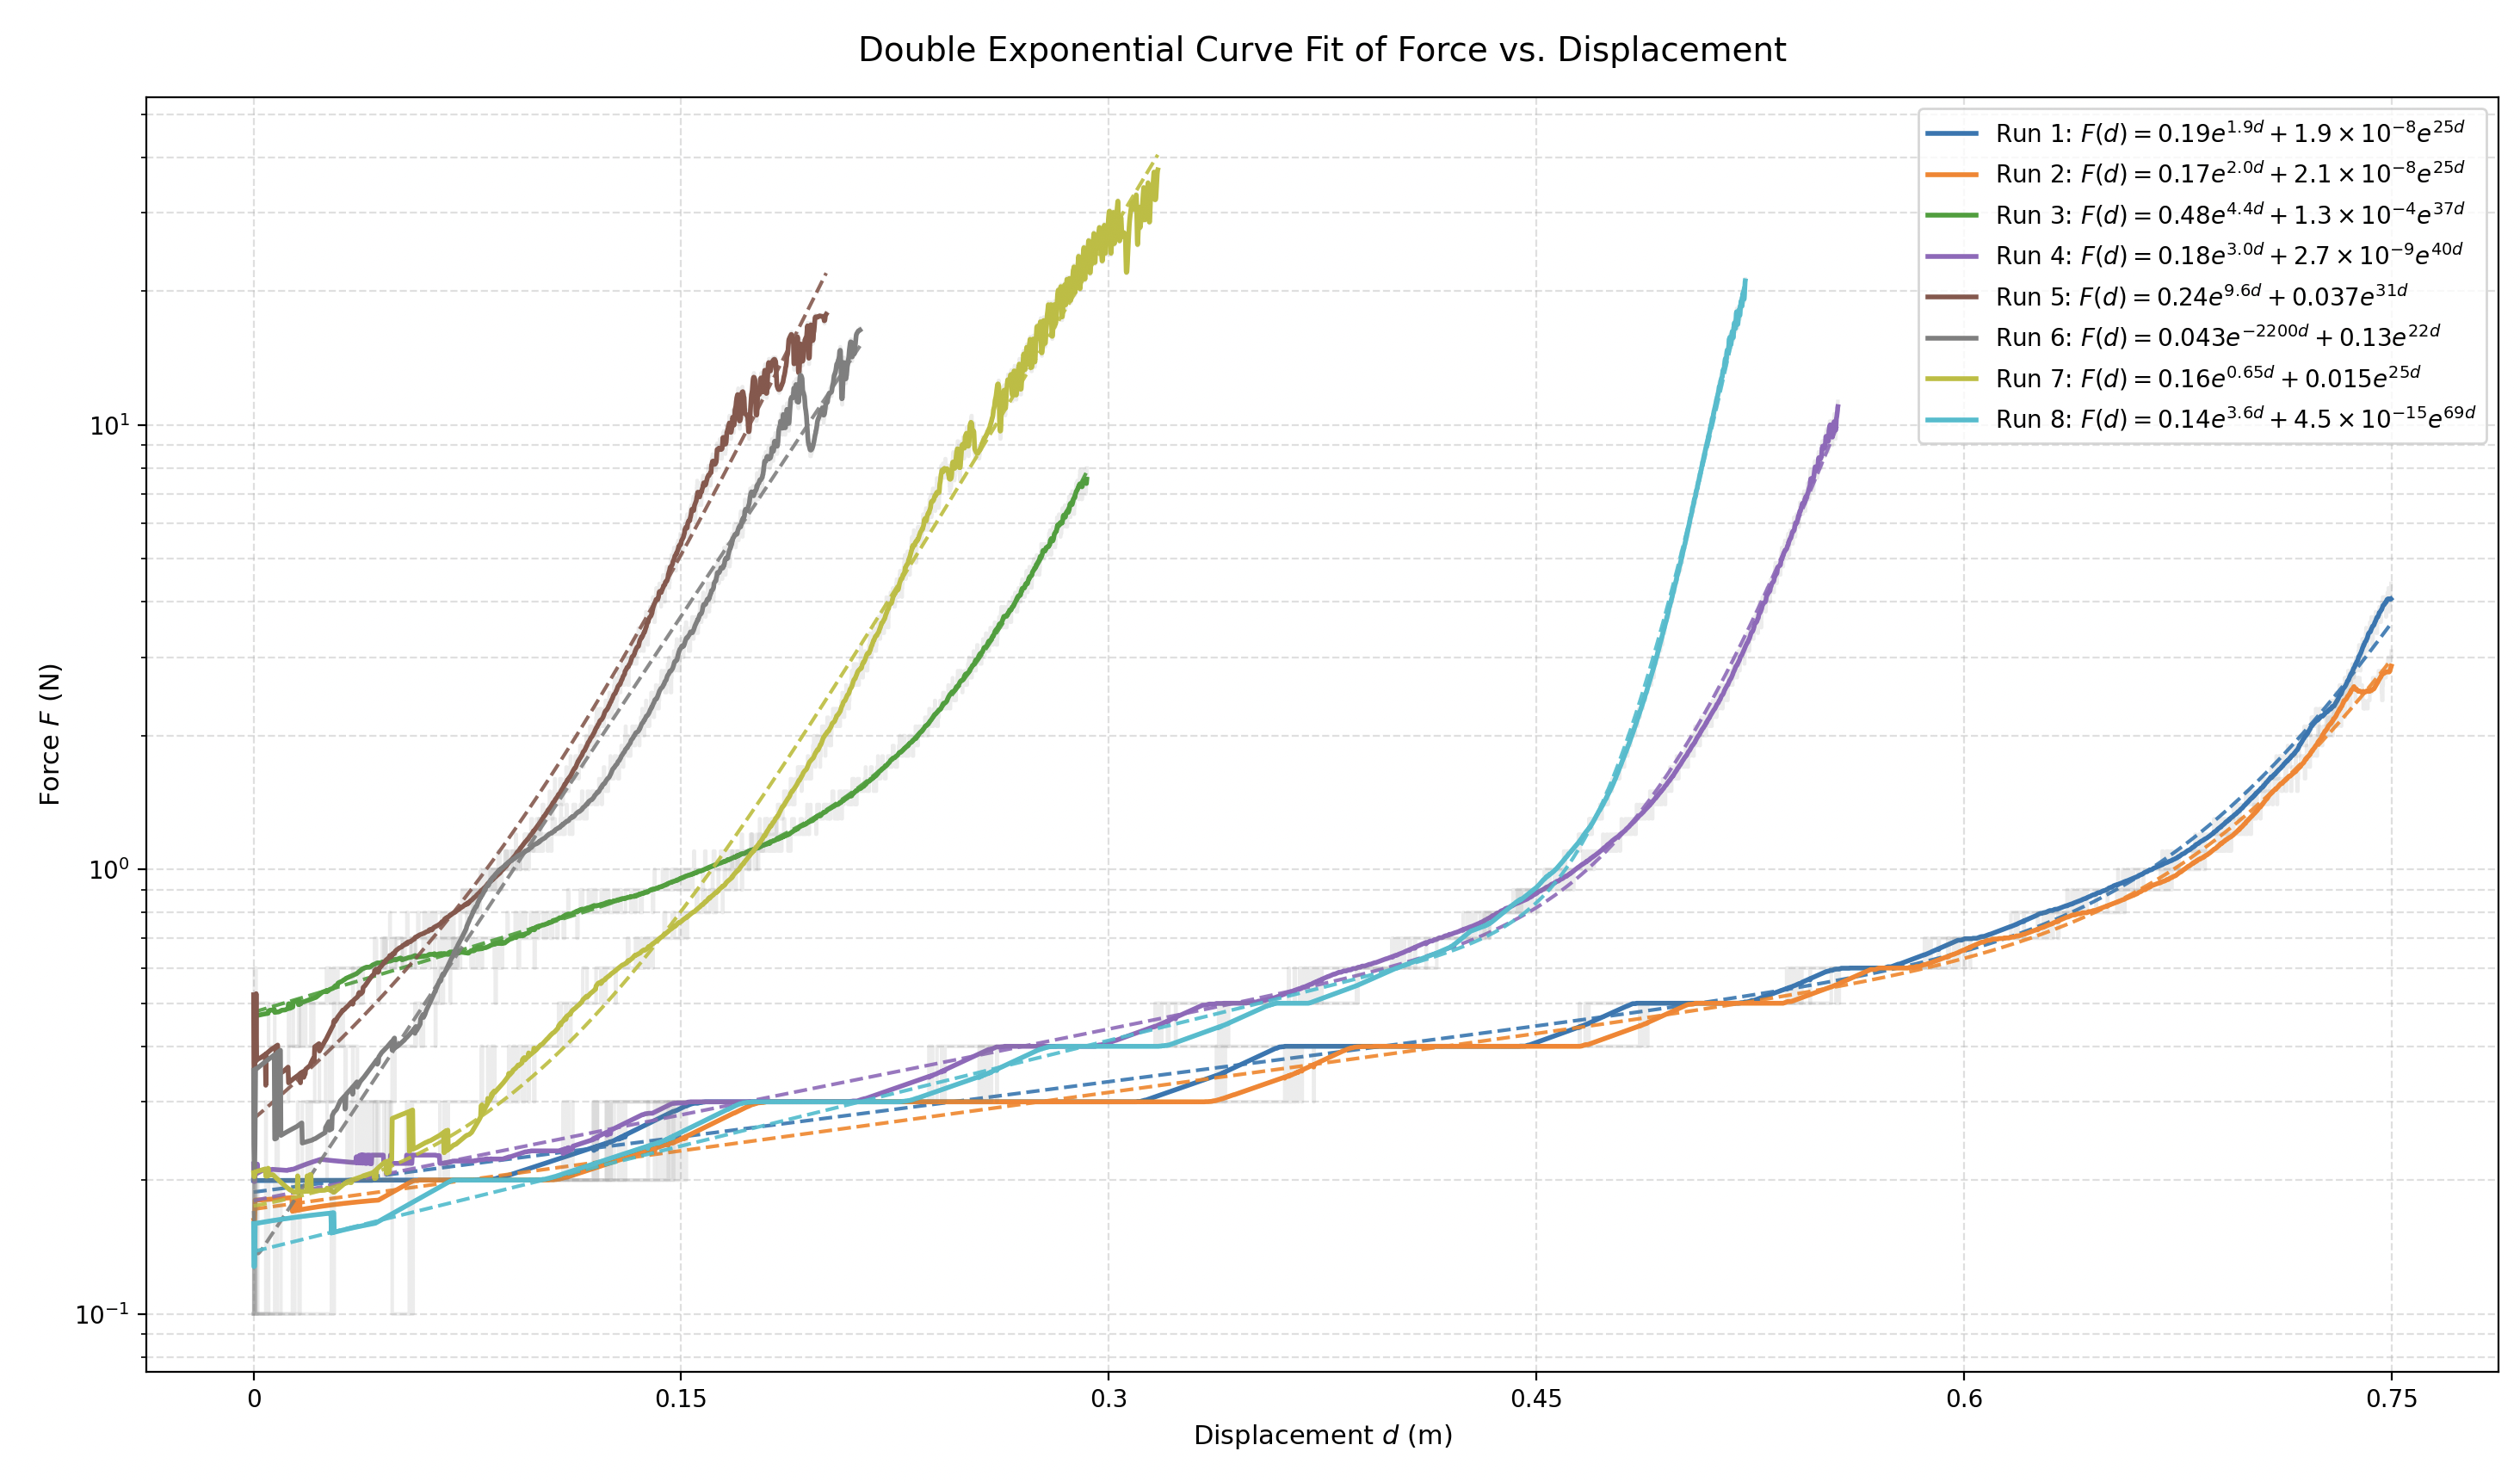
\includegraphics[width=\textwidth]{figs/instron_plot.png}
    \caption{Instron force-displacement data, with raw quantized data (grey), smoothed data (solid colored), and curve fit (dashed colored).}\label{fig:yoyo}
\end{figure}

\end{document}